\section{Completeness tests}
For the smoothed seismicity method, completeness of each magnitude in the catalog is an important factor. In order to determine the catalog completeness, according to \citet{Frankel1995}, we made plots of the cumulative number of events against time for different regions.   Fig.~\ref{fig:comptest} shows the completeness of data for each magnitude threshold in three different regions.
A uniform rise of cumulative number of earthquake in each magnitude big, defines the threshold for catalog completeness. Fig.~\ref{fig:comptest} (a,b,c) show the plot of earthquake magnitude with time. Fig.~\ref{fig:comptest}(d-o) present the cumulative number of earthquake with magnitude, in defined ranges. We define a completeness of each magnitude range at a time which the cumulative number of earthquake increase linearly with time. These times which presents the completeness of the catalog of each region for different moment magnitude are represented at Table 1. We assume the catalog for earthquakes with magnitude greater than $M_w=7$ is complete from the first historical earthquake report. 

\begin{figure} [H]
\centering
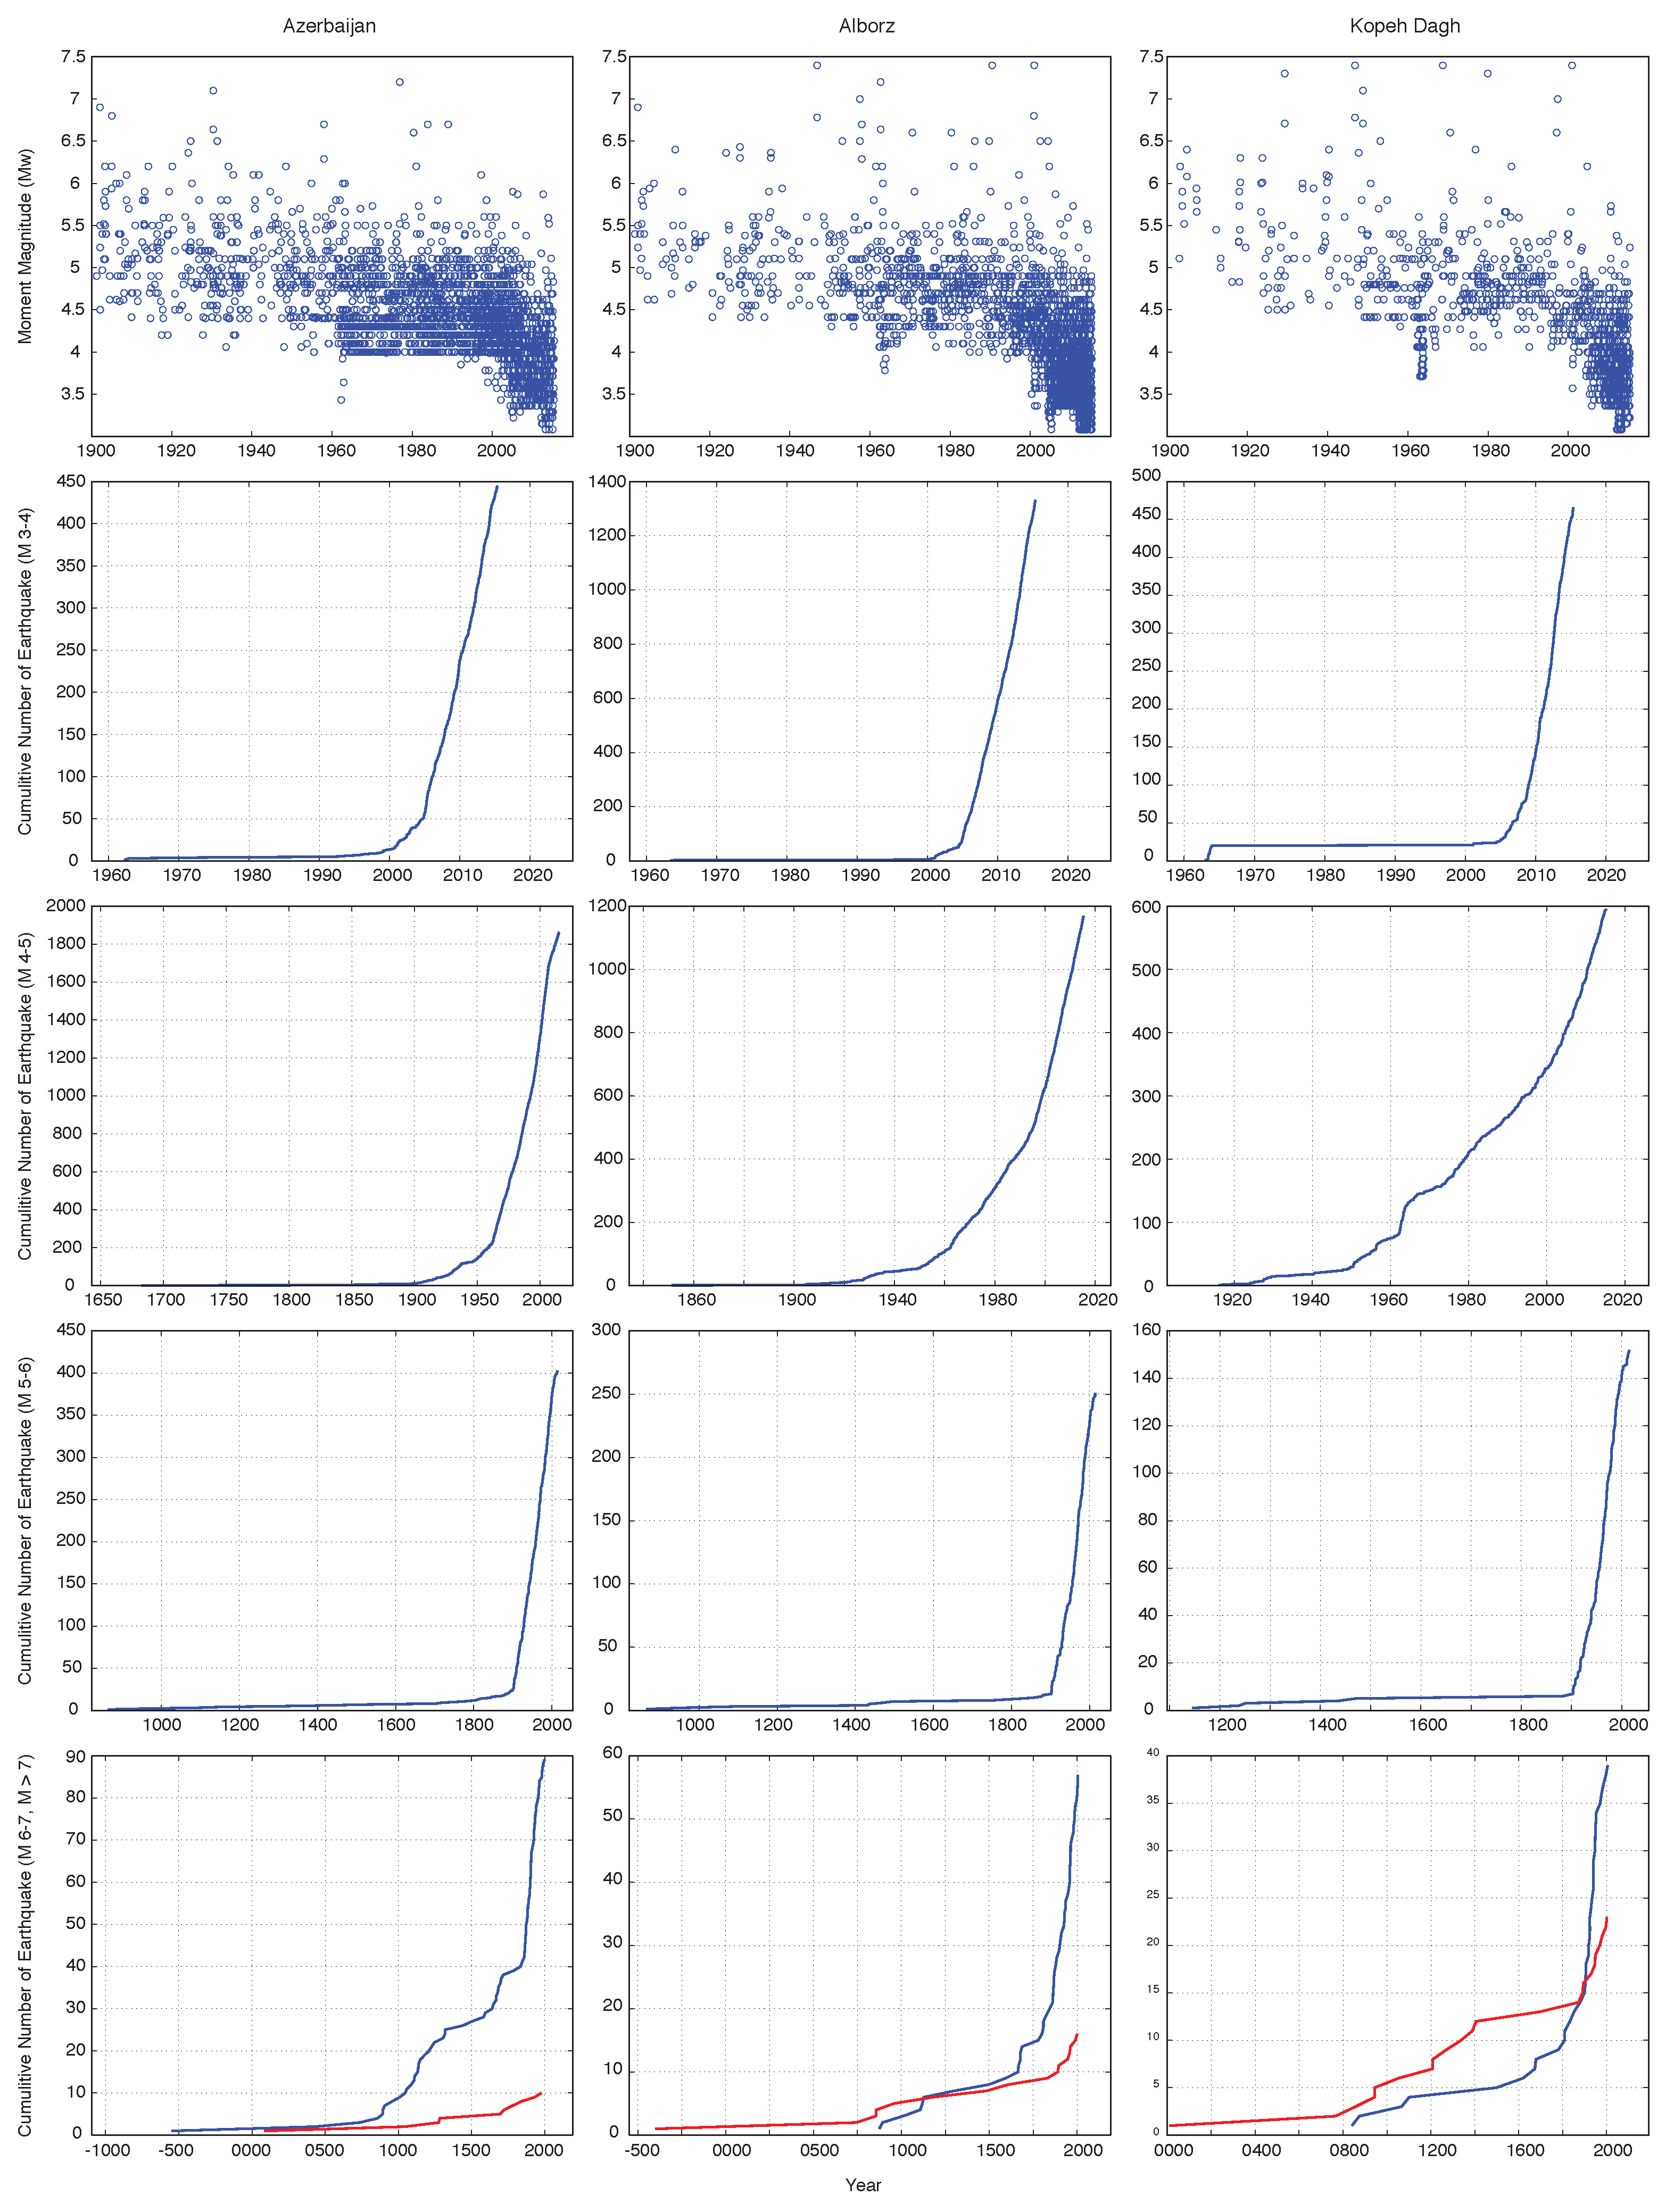
\includegraphics[scale=0.3]{figures/pdf/Figure4.pdf} 
\caption{Completeness test for earthquakes occurred in the three study regions. Red lines represent $M_w > 7$ }
\label{fig:comptest}
\end{figure}



\begin{table}[h]
\centering
\caption{Completeness threshold of three tectonic seismic regions.}
\begin{tabular}{cccc}
 ~           & Azerbaijan & Alborz & Kopeh Dagh \\ \hline
3-4         & 2004       & 2004   & 2005       \\ \hline
4-5         & 1960       & 1960   & 1960       \\ \hline
5-6         & 1900       & 1900   & 1900       \\ \hline
6-7         & 1844       & 1809   & 1810         \\ \hline
7 $< $    &  85          & -400    & 10         \\ \hline
\end{tabular}
\end{table}

